\section{Durchf\"uhrung}
\label{sec:durchfuehrung}
\subsection{Aufbau}
F\"ur die durchzuf\"uhrenden Versuche stehen vier verschiedene Supraleiter-Proben und drei Seltene-Erden-Permanentmagnete zur Verf\"ugung.
In den aufgef\"uhrten Tabellen (\ref{tab:probenSL}) und (\ref{tab:probenM}) sind einige wichtige Kenndaten der Supraleiter-Proben und Magnete aufgelistet.
\begin{table}
	\centering
	\caption{Die Supraleiter-Proben.}
\begin{tabular}{|c|lll|}
	\hline
	{SL} & {Material} & {Form} & {Bemerkung} \\
	\hline
	\#1 & $Bi_2Sr_2Ca_2Cu_3O_10$ & Stab & mit Silberkontaktflächen \\
	\#2 & $YBa_2Cu_3O_7$ & d\"unne Scheibe & polykristallin; geringe kritische Stromstärken \\
	\#3 & YBCO-Einkristall & dicke Scheibe & hohe kritische Stromstärken \\
	\#4 & $Bi_2Sr_2Ca_2Cu_3O_10$ & Ring &  \\
	\hline
\end{tabular}
\label{tab:probenSL}
\end{table}
\begin{table}
	\centering
	\caption{Die Seltene-Erden-Permanentmagnete.}
\begin{tabular}{|c|cc|}
	\hline
	{M} & {Material} & {(Durchmesser \times \, H\"ohe) / mm} \\
	\hline
	\#M1 & NdFeB-Magnet & 4 \times \, 1,5 \\
	\#M2 & NdFeB-Magnet & 15 \times \, 5 \\
	\#M3 & NdFeB-Magnet & 12,6 \times \, 12,6 \\
	\hline
\end{tabular}
\label{tab:probenM}
\end{table}

In Abbildung (\ref{abb:aufbau}) ist beispielhaft der Versuchsaufbau f\"ur den dritten Versuchsteil zu sehen.
Mittig befindet sich ein gro{\ss}es Styroporbeh\"ahlter (wei{\ss}), in welchem sich das fl\"ussige Stickstoff befindet, womit die Proben gek\"uhlt werden.
In dem kleineren Styroporbeh\"ahlter (blau) wird der Supraleiter platziert.
Zum Aufbau geh\"ohren au{\ss}erdem eine Stromquelle (Rigol DP821A), ein Nanovoltmeter (Hioki DM7275-01), verschiedene Temperatursensoren und eine transversalen USB-Hall-Sonde .
Die Stromquelle kann einen variablen Strom von einigen mA bis hin zu 1 A durch SL \#1 flie{\ss}en lassen.
Die abfallende Spannung kann mittels dem Nanovoltmeter bestimmt werden.
Mit hilfe eines Multimeters werden die Temperatursensoren ausgelesen.
\begin{figure}[hbtp]
	\centering
	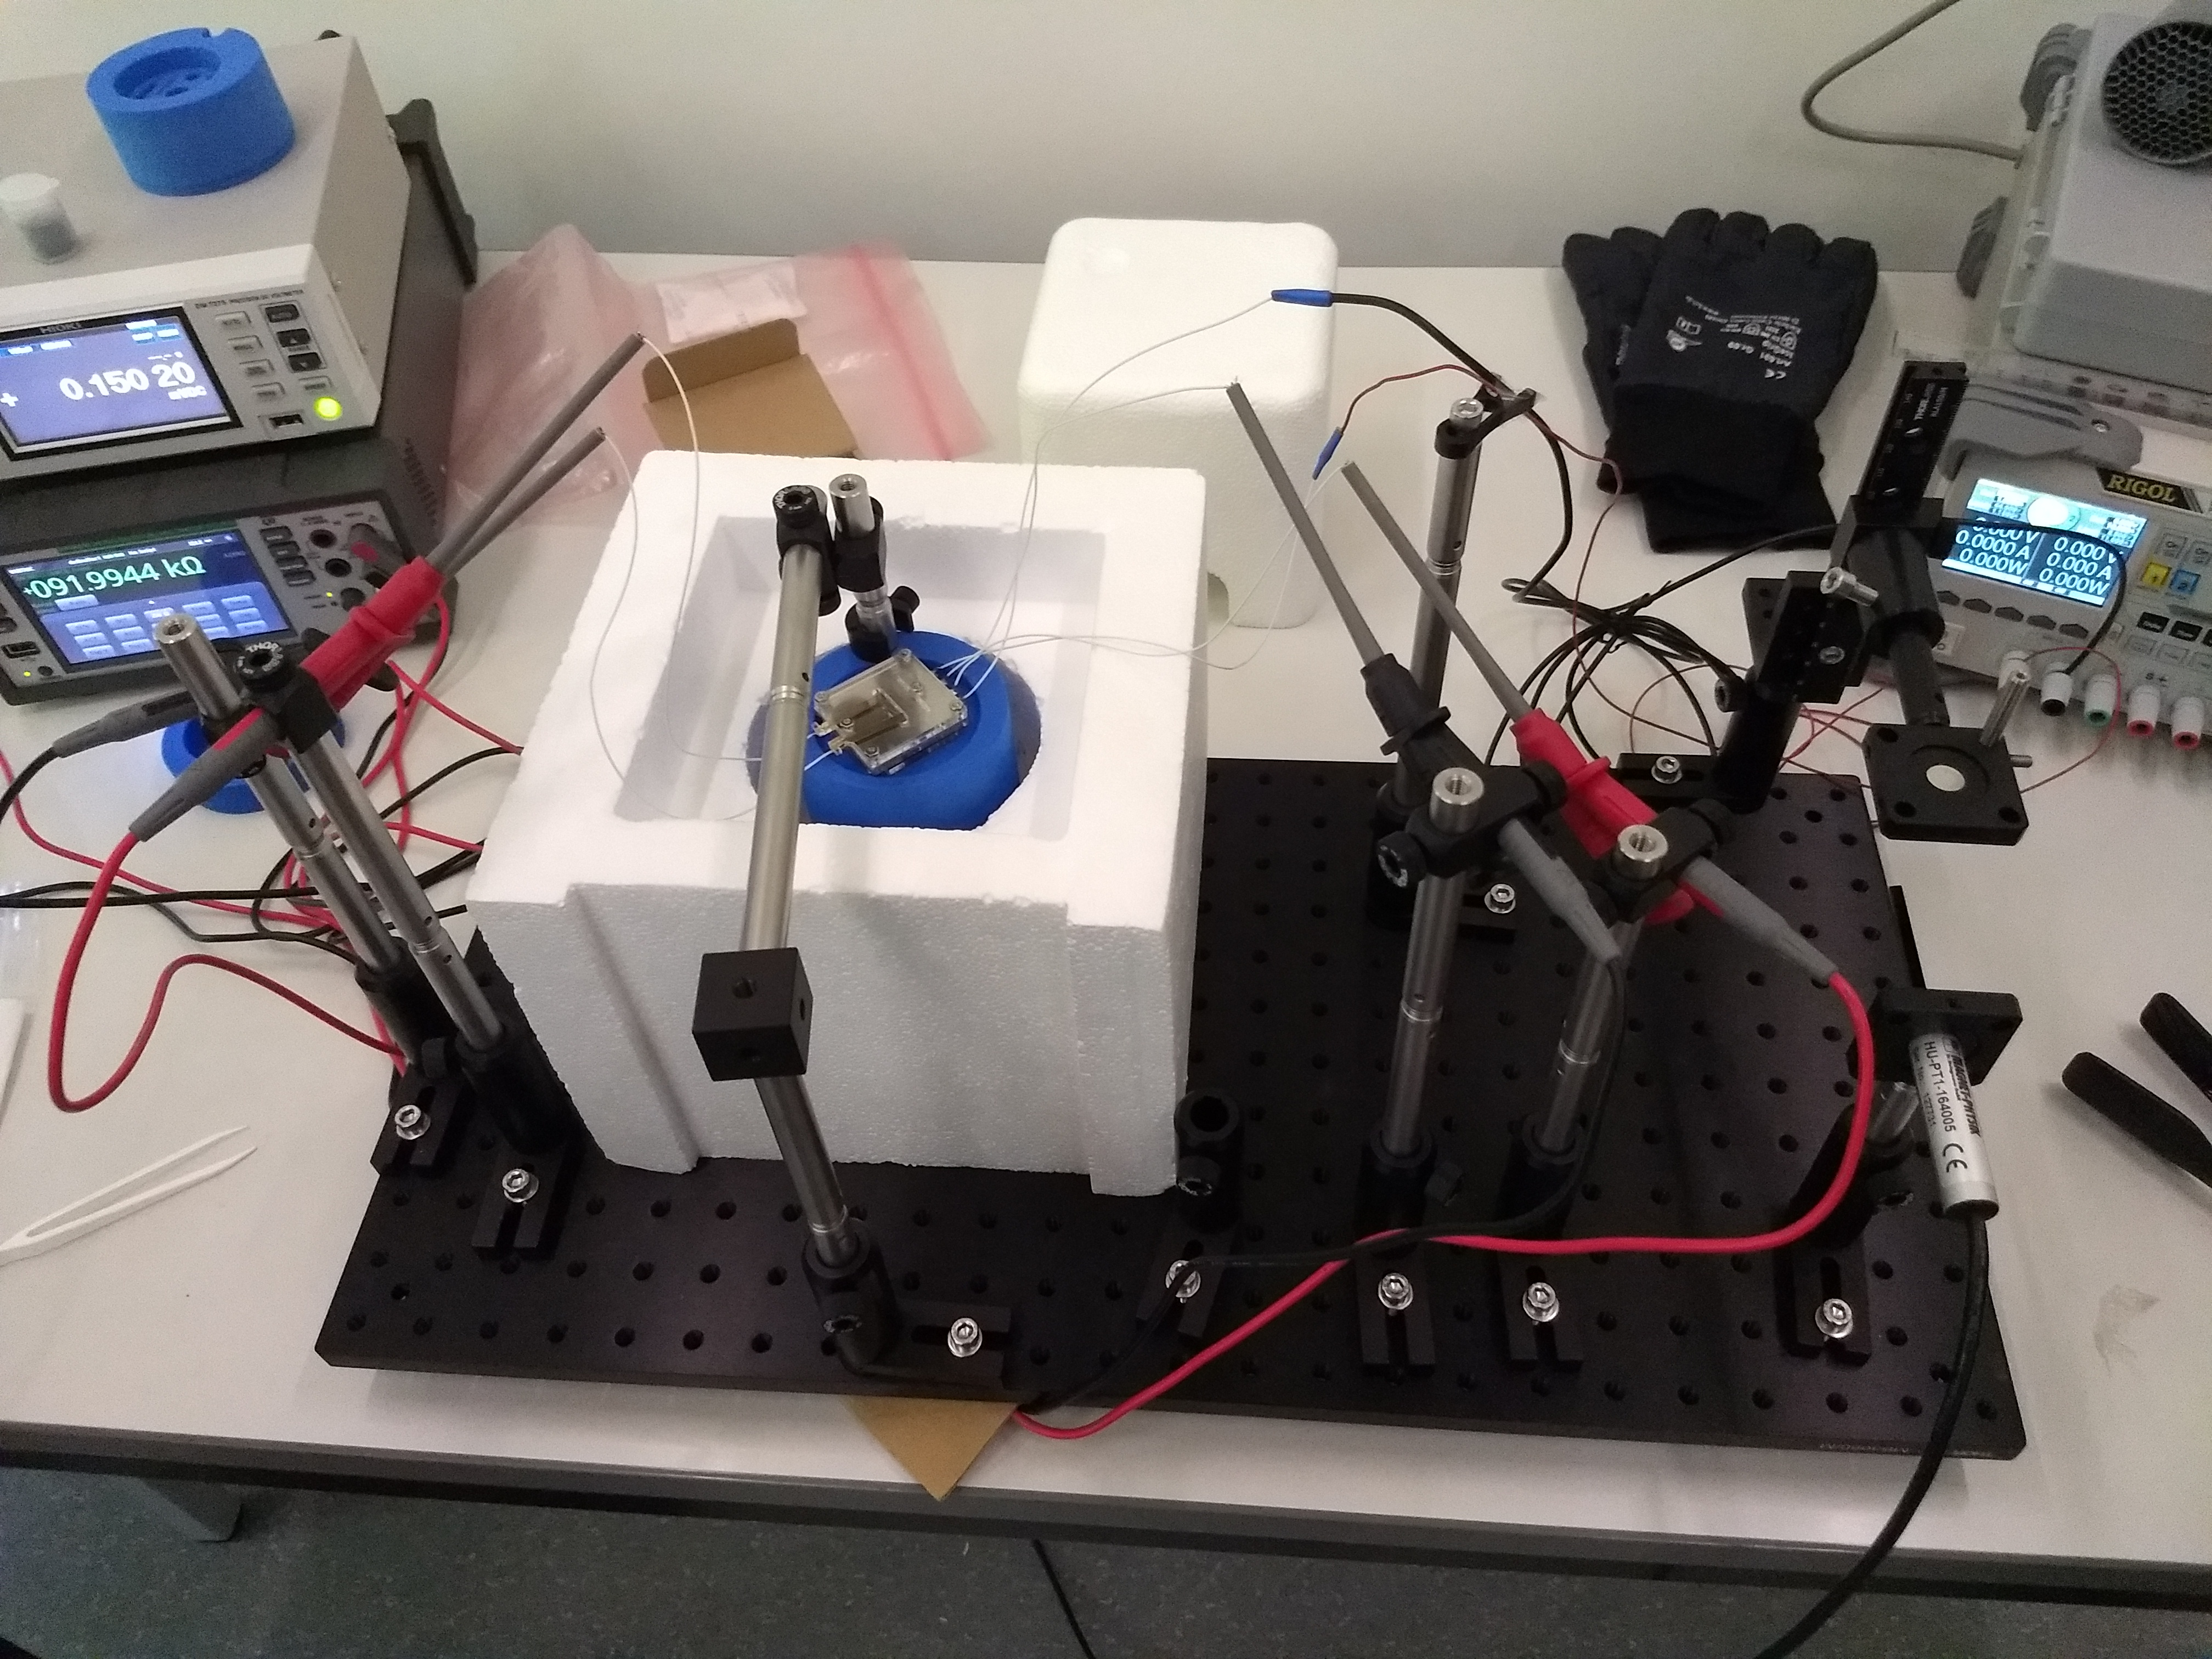
\includegraphics[width=0.6\textwidth]{Plots/aufbau_SL.jpg}
	\caption{Zu sehen ist hier ein Versuchsaufbau f\"ur die dritte Messreihe. In dem blauen Styroporbeh\"ahlter befindet sich der SL \#1, welcher \"uber mehrere Kabel mit der Stromquelle verbunden ist.}
	\label{abb:aufbau}
\end{figure}
Zus\"atzlich befindet sich auch ein Heißluftfön neben dem Versuchsaufbau.
Dieser wird ben\"otigt um die feuchtigkeitsempfindlichen Supraleiter-Proben nach jeder Messung wieder zu trocknen.

\subsection{Experiment}
Bevor es mit den eigentlichen Messungen losgeht, wird sich mit den Supraleiter vertraut gemacht.
Hierbei liegt der Schwerpunkt auf der Beobachtung und Beschreibung des Meißner-Ochsenfeld-Effekts.
Daf\"ur wird \#M1 auf den abgekühlten SL \#2 platziert.
Für Rotations- und Suspensionsexperimente wird die Konstruktions von SL \#3, einem Abstandsplättchen und \#M3 zusammen in einem Styroporbehältnis mit fl\"ussig Stickstoff gek\"uhlt. \\

In den ersten zwei Messreihen wird die kritische Temperatur $T_C$ einmal mit Hilfe des Meißner-Ochsenfeld-Effekt und ein zweites Mal mittels einer 4-Punkt-Messung bestimmt.
F\"ur erstere Messreihe wird die der zeitliche Verlauf der Spannung $U(t)$ und der Temperatur $T(t)$ aufgenommen.
Dieser Versuch wird mit SL \#2 und \#M1 durchgef\"uhrt.
Die 4-Punkt-Messung wird an SL \#1 vorgenommen.
Der Aufbau f\"ur diese Messreihe ist in Abbilung (\ref{abb:aufbau}) dargestellt.
Die Stromst\"arke wird hinf\"ur auf $0,6 \,$A eingestellt.
Gemessen wird der Widerstand $R$ des Platin-Temperatursensors und die Spannung $U_{SL}$ am SL \#1.
Sobald der Widerstand $R$ einen Wert von ca. $50 \, \Omega$ annimmt, wird die Messung beendet.
Untersucht wird das ganze mit und ohne Einfluss eines externen Magnetfeldes.
Als externes Magnetfeld wird \#M3 verwendet. \\

In einer weiteren Messreihe wird die kritischen Stromstärke $I_C$ vom SL \#1 abgesch\"atzt.
Die $R_{SL}(T)$ Abhängigkeit wird f\"ur fünf verschiedene Stromstärken aufgenommen.
% um daraus auf die kritische Temperatur zu schlie{\ss}en.
Die f\"unf Messungen weerden jeweils mit und ohne externex Magnetfeld durchgef\"uhrt. \\


Als letztes wird der induzierten Strom $I_{ind}$ an dem Supraleitenden Ring SL \#4 abgesch\"atzt.
der SL \#4 wird in einem Styroporbehälter, welcher mit fl\"ussigem Stickstoff gef\"ullt ist, abgek\"uhlt.
Mittels dem Permanentmagneten \#M3 wird ein Strom in dem Ring induziert.
Um ein m\"oglichst genaues Messergebnis zu erhalten, wird der Ring schnell aus dem Behälter entfernt und da Magnetfeld wird gemessen.